\documentclass[a4paper,14pt]{extreport} % формат документа

\usepackage{amsmath}
\usepackage{cmap} % поиск в ПДФ
\usepackage[T2A]{fontenc} % кодировка
\usepackage[utf8]{inputenc} % кодировка исходного текста
\usepackage[english,russian]{babel} % локализация и переносы
\usepackage[left = 2cm, right = 1cm, top = 2cm, bottom = 2 cm]{geometry} % поля
\usepackage{listings}
\usepackage{graphicx} % для вставки рисунков
\usepackage{amsmath}
\usepackage{float}
\usepackage{multirow}
\graphicspath{{pictures/}}
\usepackage{amsfonts}
\usepackage{breqn}
\DeclareGraphicsExtensions{.pdf,.png,.jpg}
\newcommand{\anonsection}[1]{\section*{#1}\addcontentsline{toc}{section}{#1}}

\renewcommand{\thesection}{\arabic{section}}

\begin{document}
\begin{titlepage}

    \begin{table}[H]
        \centering
        \footnotesize
        \begin{tabular}{cc}
            \multirow{8}{*}{
\includegraphics[scale=0.35]{bmstu.jpg}}
            & \\
            & \\
            & \textbf{Министерство науки и высшего образования Российской Федерации} \\
            & \textbf{Федеральное государственное бюджетное образовательное учреждение} \\
            & \textbf{высшего образования} \\
            & \textbf{<<Московский государственный технический} \\
            & \textbf{университет имени Н.Э. Баумана>>} \\
            & \textbf{(МГТУ им. Н.Э. Баумана)} \\
        \end{tabular}
    \end{table}

    \vspace{-2.5cm}

    \begin{flushleft}
        \rule[-1cm]{\textwidth}{3pt}
        \rule{\textwidth}{1pt}
    \end{flushleft}

    \begin{flushleft}
        \small
        ФАКУЛЬТЕТ
        \underline{<<Информатика и системы управления>>\ \ \ \ \ \ \ 
        \ \ \ \ \ \ \ \ \ \ \ \ \ \ \ \ \ \ \ \ \ \ \ \ \ \ \ \ \ \ \ 
    \ \ \ \ \ \ \ \ \ \ \ \ \ \ \ } \\
        КАФЕДРА
        \underline{<<Программное обеспечение ЭВМ и
        информационные технологии>>
        \ \ \ \ \ \ \ \ \ \ \ \ \ \ \ \ \ \ \ \ }
    \end{flushleft}

    \vspace{2cm}

    \begin{center}
        \textbf{Домашняя работа № 1} \\
        \vspace{0.5cm}
    \end{center}

    \vspace{5cm}

    \begin{flushleft}
        \begin{tabular}{ll}
            \textbf{Дисциплина} & Математическая статистика.  \\
            \textbf{Студент} & Сиденко А.Г. \\
            \textbf{Группа} & ИУ7-63Б \\
            \textbf{Вариант} & 22 \\
            \textbf{Оценка (баллы)} & \\
            \textbf{Преподаватель} & Власов П.А.   \\
        \end{tabular}
    \end{flushleft}

    \vspace{4cm}

   \begin{center}
        Москва, 2020 г.
    \end{center}

\end{titlepage}

\section{Задача 1 (Предельные теоремы теории вероятностей)}

\hfill

\textbf{Условие}

Известно, что 80\% изготовленных заводом электроламп выдерживают гарантийный срок службы. Найти вероятность того, что в партии из 500 электроламп число выдержавших гарантийный срок службы находится в пределах от 380 до 420. Использовать неравенство Чебышева и интегральную теорему Муавра-Лапласа.

\hfill

\textbf{Решение}

\begin{enumerate}
\item С использованием неравенства Чебышева. 

$$A=\{\text{Лампа выдержала гарантийный срок}\}$$

$$P(A)=0.8$$

Так как отдельные испытания независимы, то значит испытания проводятся по схеме Бернулли $n = 500$, вероятность успеха $p = 0.8$.

Тогда

$$K_n - \text{число успехов в расмотренной серии} $$

$$K_n \sim B(n,p)$$

$$MK_n=n\cdot p=500\cdot 0.8=400$$

$$DK_n=n\cdot q\cdot p=n\cdot(1-p)\cdot p=500\cdot0.2\cdot0.8=80$$

\begin{multline*}
P\{380\le K_n \le 420\}=P\{380-400\le K_n-MK_n\le 420-400\}=\\=P\{-20\le K_n-MK_n\le 20\}=P\{|K_n-MK_n|\le 20\} \ge 1 -\frac{DK_n}{\epsilon^2}=\\=1-\frac{80}{20\cdot 20} =\frac{4}{5}=0.8
\end{multline*}

\item С использованием теоремы Муавра-Лапласа. 

\begin{multline*}
P\{K_1\le K_n\le K_2\}\approx \Phi_0\big(\frac{K_2-n\cdot p}{\sqrt{n\cdot p \cdot q}}\big) - \Phi_0\big(\frac{K_1-n\cdot p}{\sqrt{n\cdot p \cdot q}}\big) = \Phi_0\big(\frac{420-500\cdot 0.8}{\sqrt{500\cdot 0.8 \cdot 0.2}}\big)-\\-\Phi_0\big(\frac{380-500\cdot 0.8}{\sqrt{500\cdot 0.8 \cdot 0.2}}\big)=2\cdot\Phi_0\big(\frac{20}{\sqrt{80}}\big)=2\cdot\Phi_0\big(\frac{20}{4\sqrt{5}}\big)=2\cdot\Phi_0\big(\sqrt{5})=2\cdot 0.4861=\\=0.9722
\end{multline*}

\end{enumerate}

\hfill

\textbf{Ответ:}
\begin{enumerate}
\item С использованием неравенства Чебышева. $P\{380\le K_n \le 420\}\ge0.8$
\item С использованием теоремы Муавра-Лапласа. $P\{380\le K_n \le 420\}=0.9722$
\end{enumerate}

\section{Задача 2 (метод моментов)}

\hfill

\textbf{Условие}

С использованием метода моментов для случайной выборки $\vec X = (X_1, . . . , X_n)$ из генеральной совокупности $X$ найти точечные оценки указанных параметров заданного закона распределения.

Закон распределения: $$f_X(x)=\frac{1}{4^{\Theta}\Gamma(\Theta)}x^{\Theta -1}e^{-\frac{x}{4}}, x>0$$

\hfill

\textbf{Решение}

\begin{enumerate}
\item 

Неизвестный параметр: $\Theta \Rightarrow r=1$

Следовательно, найдем момент 1-ого порядка. 

$$
f_X(x)=\frac{1}{4^{\Theta}\Gamma(\Theta)}x^{\Theta -1}e^{-\frac{x}{4}} = \frac{(\frac{1}{4})^\Theta x^{\Theta-1}e^{-\frac{1}{4}\cdot x}}{\Gamma(\Theta)}
$$

\begin{multline*}
MX = \int_{-\infty}^{+\infty}x\cdot f(x) dx=\int_0^{+\infty}\frac{x(\frac{1}{4})^\Theta x^{\Theta-1}e^{-\frac{1}{4}\cdot x}}{\Gamma(\Theta)}dx=
\begin{vmatrix}
\text{Замена:}\\
t=\frac{x}{4},~dx=4dt\\
x=4t\\
\end{vmatrix}
=\\
= \int_0^{+\infty} \frac{(4t)^\Theta (\frac{1}{4})^\Theta e^{-t}}{\Gamma(\Theta)}4 dt =\frac{4}{\Gamma(\Theta)}\underbrace{\int_0^{+\infty}t^\Theta e^{-t}dt}_{\Gamma(\Theta+1)}=\frac{4\Gamma(\Theta+1)}{\Gamma(\Theta)}=
\\ =\begin{vmatrix}
\text{По свойству}\\
\text{гамма-распределения}\\
\end{vmatrix}
= \frac{4\Gamma(\Theta)\Theta}{\Gamma(\Theta)}=4\Theta
\end{multline*}

\item Приравняем теоретические моменты к их выбранным аналогам, найдем неизвестный параметр

$$MX=\overline x=4\Theta \Rightarrow \Theta=\frac{\overline x}{4}$$

\end{enumerate}

\hfill

\textbf{Ответ:} $ \Theta=\frac{\overline x}{4}$

\section{Задача 3 (метод максимального правдоподобия)}

\hfill

\textbf{Условие}

С использованием метода максимального правдоподобия для случайной выборки $\vec X = (X_1, . . . , X_n)$ из генеральной совокупности $X$ найти точечные оценки указанных параметров заданного закона распределения. Вычислить выборочные значения найденных оценок для выборки $\vec x_5 =  (x_1, . . . , x_5)$.

Закон распределения: $$f_X(x)=\frac{\Theta^5}{4!}x^4 e^{-\Theta x}, x>0$$

Выборка $\vec x_5 = (7,4,11,5,3)$ 

\hfill

\textbf{Решение}

\begin{enumerate}

\item

\begin{multline*}
\alpha(x_1,..x_n,\Theta)=f(x_1,\Theta)\cdot ... \cdot f(x_n,\Theta)=\frac{\Theta^5}{4!}x_1^4 e^{-\Theta x_1}\cdot ... \cdot \frac{\Theta^5}{4!}x_n^4 e^{-\Theta x_n}=\\
=\bigg(\frac{\Theta^5}{4!}\bigg)^n \cdot e^{-\Theta \sum_{i=1}^{n}x_i}\cdot (x_1^4\cdot ... \cdot x_n^4)
\end{multline*}

\item

\begin{multline*}
\ln \alpha= n\ln\frac{\Theta^5}{4!}  -\Theta \sum_{i=1}^{n}x_i + \ln(x_1^4\cdot ... \cdot x_n^4)=\\=5n\ln\Theta-n\ln4!-\Theta \sum_{i=1}^{n}x_i + \ln(x_1^4\cdot ... \cdot x_n^4) \rightarrow max
\end{multline*}

\item

Необходимое условие экстремума:
$$\frac{\partial \ln\alpha}{\partial \Theta}=-\sum_{i=1}^{n}x_i + \frac{5n}{\Theta}$$

$$\Theta=\frac{5n}{\sum_{i=1}^{n}x_i}=\frac{5}{\overline x}$$

$$\hat \Theta = \frac{5}{\overline x}$$

Достаточное условие экстремума:

\begin{multline*}
\frac{\partial^2 \ln\alpha}{\partial \Theta^2}=-\frac{5n}{\Theta^2}\bigg|_{\Theta = \hat \Theta = \frac{5}{\overline x}}=-\frac{5n\overline x^2}{25}=-\frac{n\overline x^2}{5}=
\begin{vmatrix}
\overline x^2\ge 0\\
n > 0
\end{vmatrix} \Rightarrow -\frac{n\overline x^2}{5} < 0  \Rightarrow \\ \Theta = \hat \Theta - \text{Точка максимума}
\end{multline*}

\item Вычислим выборочные значения найденных оценок для выборки 

$\vec x_5 = (7,4,11,5,3)$. 

$$\hat \Theta = \frac{5\cdot 5}{x_1+...+x_5}=\frac{25}{7+4+11+5+3}=\frac{25}{30}=\frac{5}{6}$$
\end{enumerate}

\hfill

\textbf{Ответ:}

\begin{enumerate}
\item $\hat \Theta = \frac{5}{\overline x}$
\item $\hat \Theta =\frac{5}{6}$
\end{enumerate}

\section{Задача 4 (доверительные интервалы)}

\hfill

\textbf{Условие}

После n = 8 измерений давления в баке с горючим получены следующие результаты: 3.25, 2.82, 3.07, 3.12, 2.93, 2.87, 3.09, 3.17. Считая ошибки измерений подчиненными нормальному закону, построить 90\%-ные доверительные интервалы для математического ожидания и среднего квадратичного отклонения давления в баке.

\hfill

\textbf{Решение}

\hfill

\begin{enumerate}
\item Пусть $X$ -- случайная величина, принимающая значения давления в баке. 

Необходимо построить доверительные интервалы для математического ожидания и среднего квадратичного отклонения давления в баке.

\item Построим доверительный интервал для математического ожидания $\theta$. 

Так как среднеквадратичное отклонение неизвестно используем центральную статистику. 

$$T(\vec X, \theta)=\frac{\theta-\overline X}{S(\vec X)}\sqrt{n} \sim St(n-1)$$

На рисунке изображен график функции плотности распределения статистики $T$. 

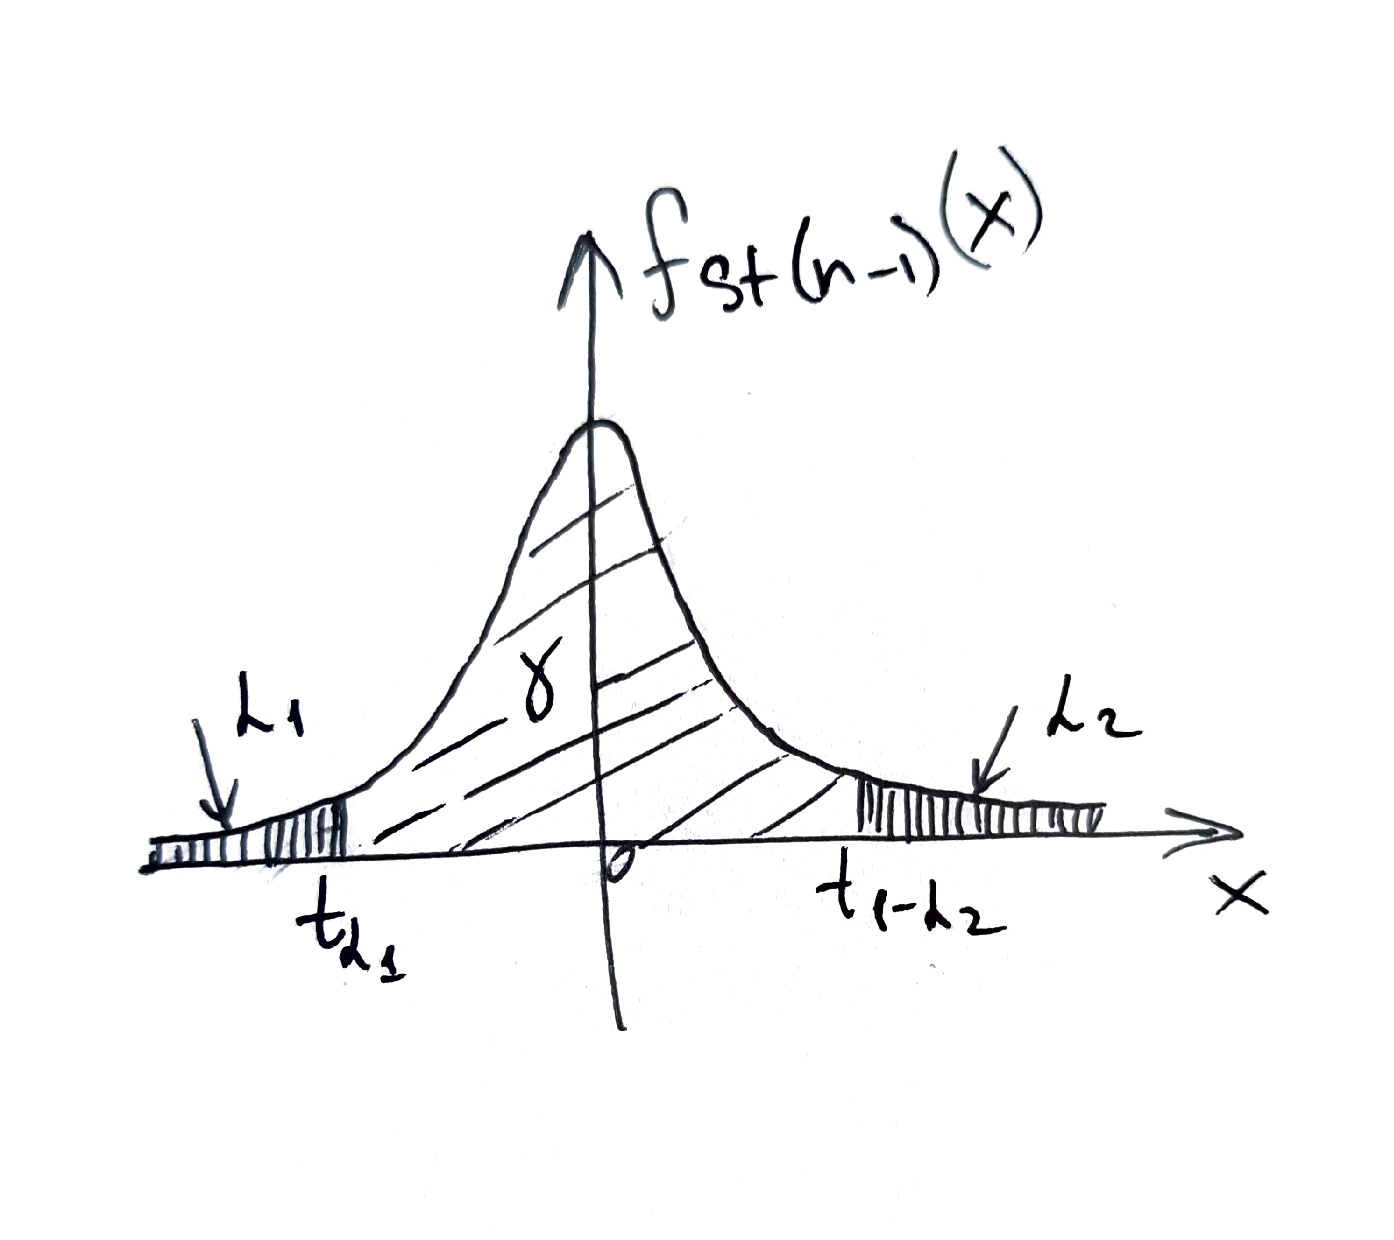
\includegraphics[scale=0.45]{2.pdf}

Следуя общей идее построения доверительных интервалов, выберем $\alpha_1,\alpha_2 > 0$ такие, что $\alpha_1+\alpha_2 = 1- \gamma$. В соответствии со свойствами непрерывных случайных величин можно записать

$$\gamma=P\{t_{\alpha_1}<T(\vec X, \theta)<t_{1-\alpha_2}\}$$

где $t_{\alpha_1},~t_{\alpha_2}$ -- квантили соответствующих уровней распределения Стьюдента с $n-1=7$ степенями свободы. 

Поскольку размах доверительного интервала обычно стараются минимизировать, то выбирают
$\alpha_1=\alpha_2=\frac{1-\gamma}{2}$ , поэтому $t_{1-\alpha_2}=t_{1-\frac{1-\gamma}{2}}=t_{\frac{1+\gamma}{2}}$. В силу симметричности функции плотности
стандартного нормального распределения заключаем, что $t_{\alpha_1}=-t_{\alpha_2}=-t_{\frac{1+\gamma}{2}}$ 

Тогда

$$\gamma=P\bigg\{-t_{\frac{1+\gamma}{2}}<\frac{\theta-\overline X}{S(\vec X)}\sqrt{n}<t_{\frac{1+\gamma}{2}}\bigg\}$$

Или

$$\gamma=P\bigg\{\overline X-\frac{t_{\frac{1+\gamma}{2}}S(\vec X)}{\sqrt{n}}<\theta<\overline X+\frac{t_{\frac{1+\gamma}{2}}S(\vec X)}{\sqrt{n}}\bigg\}$$

Тогда в качестве верхней и нижней границ $\gamma$-доверительного интервала для параметра $\theta$ могут быть использованы статистики:

$$\underline\theta(\vec X)=\overline X-\frac{t_{\frac{1+\gamma}{2}}S(\vec X)}{\sqrt{n}},$$

$$\overline\theta(\vec X)=\overline X+\frac{t_{\frac{1+\gamma}{2}}S(\vec X)}{\sqrt{n}}$$

Вычислим:

$$\overline X=\frac{1}{n}\sum_{i=1}^nX_i=\frac{3.25+2.82+3.07+3.12+2.93+2.87+3.09+3.17}{8}=3.04$$

$$\frac{1+\gamma}{2}=\frac{1+0.9}{2}=0.95$$

$$t_{\frac{1+\gamma}{2}}=t_{0.95}=1.8946$$

\begin{multline*}
S(\vec X)=\frac{1}{n-1}\sum_{i=1}^n(X_i-\overline X)^2=\frac{(3.25-3.04)^2 +(2.82-3.04)^2 +(3.07-3.04)^2+}{}\\ \frac{+(3.12-3.04)^2 +(2.93-3.04)^2 +(2.87-3.04)^2 +(3.09-3.04)^2 +(3.17-3.04)^2 }{7}\\
=0.023
\end{multline*}

$$\underline\theta(\vec X)=\overline X-\frac{t_{\frac{1+\gamma}{2}}S(\vec X)}{\sqrt{n}}=3.04-\frac{1.8946\cdot 0.023}{\sqrt{8}}=3.0246$$

$$\overline\theta(\vec X)=\overline X+\frac{t_{\frac{1+\gamma}{2}}S(\vec X)}{\sqrt{n}}=3.04+\frac{1.8946\cdot 0.023}{\sqrt{8}}=3.0554$$

\item Построим доверительный интервал для среднеквадратичного отклонения $\sigma$. 

Используем центральную статистику. 

$$T(\vec X, \sigma^2)=\frac{S^2(\vec X)}{\sigma^2}(n-1) \sim \chi^2(n-1)$$

На рисунке изображен график функции плотности распределения статистики $T$. 

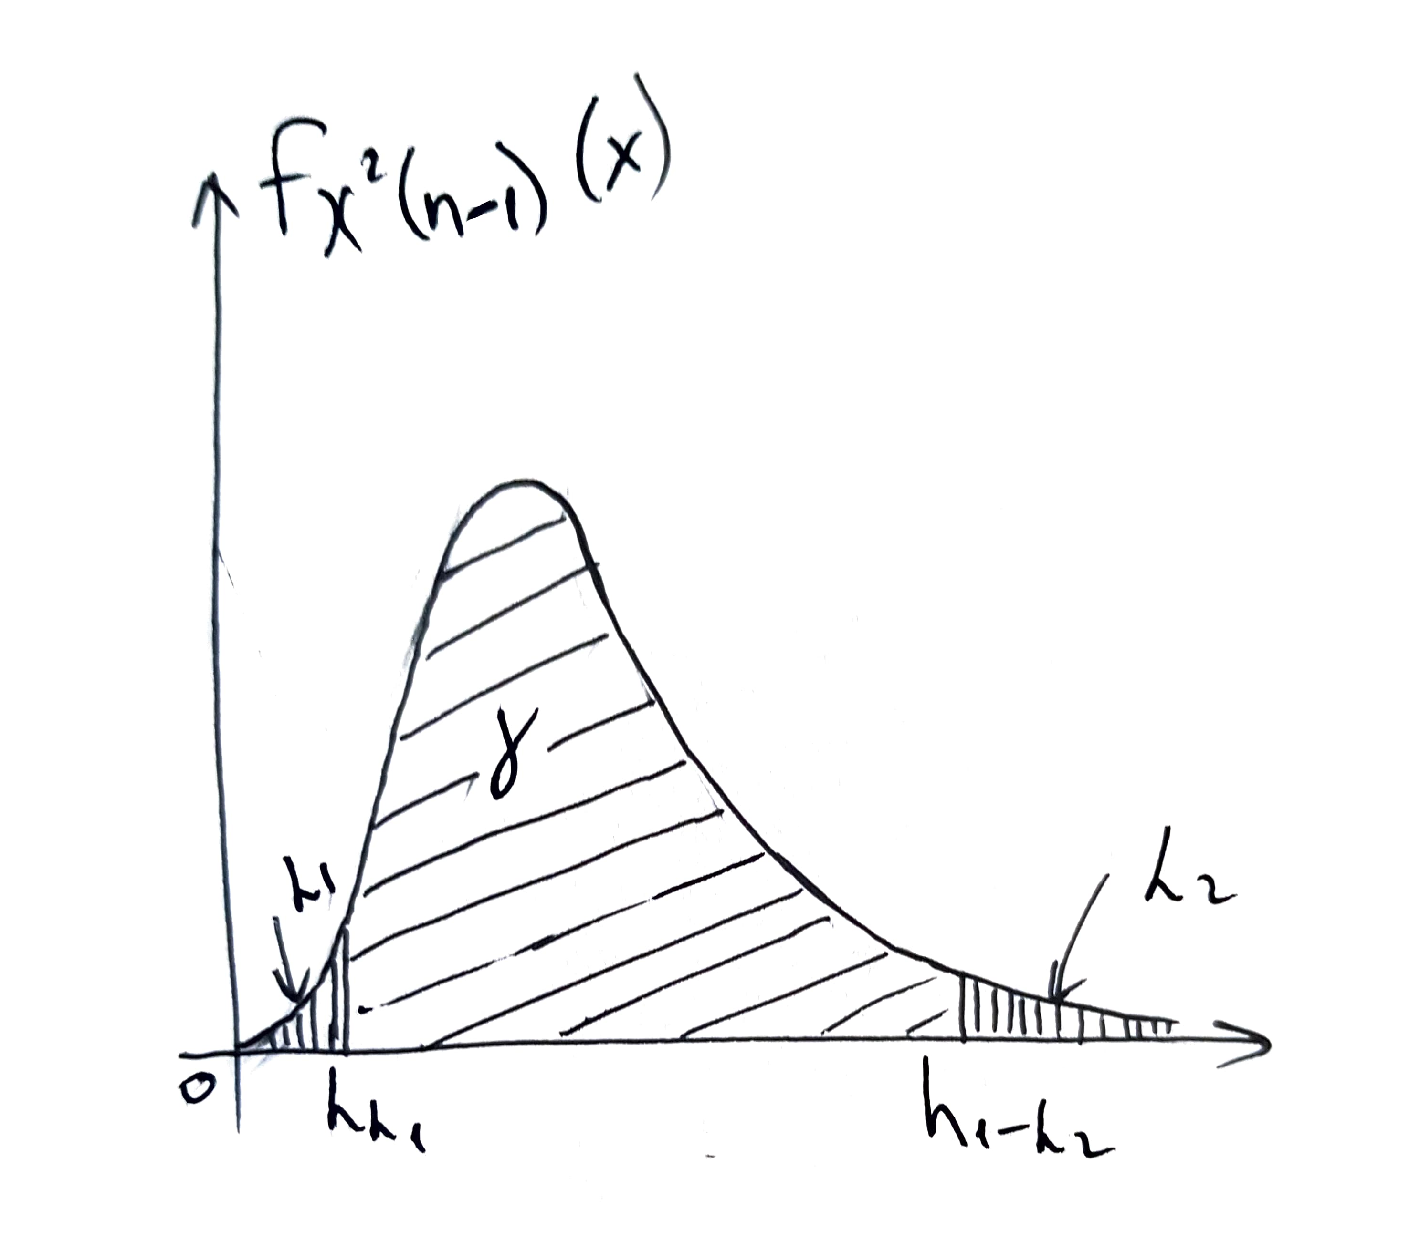
\includegraphics[scale=0.45]{1.pdf}

Следуя общей идее построения доверительных интервалов, выберем $\alpha_1,\alpha_2 > 0$ такие, что $\alpha_1+\alpha_2 = 1- \gamma$. В соответствии со свойствами непрерывных случайных величин можно записать

$$\gamma=P\{h_{\alpha_1}<T(\vec X, \sigma^2)<h_{1-\alpha_2}\}$$

где $h_{\alpha_1},~h_{\alpha_2}$ -- квантили соответствующих уровней распределения хи-квадрат с $n-1=7$ степенями свободы. 

Поскольку размах доверительного интервала обычно стараются минимизировать, то выбирают
$\alpha_1=\alpha_2=\frac{1-\gamma}{2}$ , поэтому $h_{1-\alpha_2}=h_{1-\frac{1-\gamma}{2}}=h_{\frac{1+\gamma}{2}}$. 

Тогда $h_{\alpha_1}=h_{\frac{1-\gamma}{2}},~h_{\alpha_2}=h_{\frac{1+\gamma}{2}}$, так как график функции плотности не симметричен. 

Тогда

$$\gamma=P\bigg\{h_{\frac{1-\gamma}{2}}<\frac{S^2(\vec X)}{\sigma^2}(n-1)<h_{\frac{1+\gamma}{2}}\bigg\}$$

Или

$$\gamma=P\bigg\{\frac{1}{h_{\frac{1+\gamma}{2}}}<\frac{\sigma^2}{S^2(\vec X)(n-1)}<\frac{1}{h_{\frac{1-\gamma}{2}}}\bigg\}$$

$$\gamma=P\bigg\{\frac{S^2(\vec X)(n-1)}{h_{\frac{1+\gamma}{2}}}<\sigma^2<\frac{S^2(\vec X)(n-1)}{h_{\frac{1-\gamma}{2}}}\bigg\}$$

Тогда в качестве верхней и нижней границ $\gamma$-доверительного интервала для параметра $\sigma^2$ могут быть использованы статистики:

$$\underline\sigma^2(\vec X)=\frac{S^2(\vec X)(n-1)}{h_{\frac{1+\gamma}{2}}},$$

$$\overline\sigma^2(\vec X)=\frac{S^2(\vec X)(n-1)}{h_{\frac{1-\gamma}{2}}}$$

\end{enumerate}

Вычислим:

$$\frac{1+\gamma}{2}=\frac{1+0.9}{2}=0.95$$

$$h_{\frac{1+\gamma}{2}}=h_{0.95}=14$$

$$\frac{1-\gamma}{2}=\frac{1+0.9}{2}=0.05$$

$$h_{\frac{1-\gamma}{2}}=h_{0.05}=2.17$$

\begin{multline*}
S(\vec X)=\frac{1}{n-1}\sum_{i=1}^n(X_i-\overline X)^2=\frac{(3.25-3.04)^2 +(2.82-3.04)^2 +(3.07-3.04)^2+}{}\\ \frac{+(3.12-3.04)^2 +(2.93-3.04)^2 +(2.87-3.04)^2 +(3.09-3.04)^2 +(3.17-3.04)^2 }{7}\\
=0.023
\end{multline*}

$$S^2(\vec X)=0.000529$$

$$\underline\sigma^2(\vec X)=\frac{S^2(\vec X)(n-1)}{h_{\frac{1+\gamma}{2}}}=\frac{0.000529\cdot 7}{14}=0.0002645$$

$$\overline\sigma^2(\vec X)=\frac{S^2(\vec X)(n-1)}{h_{\frac{1-\gamma}{2}}}=\frac{0.000529\cdot 7}{2.17}=0.0017$$

\textbf{Ответ:}

Доверительные интервалы уровня 0.9 для математического ожидания (3.0246, 3.0554) и среднего квадратичного отклонения (0.0002645, 0.0017) давления в баке.

\end{document}